%% LyX 2.0.6 created this file.  For more info, see http://www.lyx.org/.
%% Do not edit unless you really know what you are doing.
\documentclass[12pt,twoside,american]{report}
\usepackage[T1]{fontenc}
\usepackage[latin9]{inputenc}
\usepackage[a4paper]{geometry}
\geometry{verbose,tmargin=2cm,bmargin=2cm,lmargin=2cm,rmargin=2cm}
\setcounter{secnumdepth}{4}
\setcounter{tocdepth}{4}
\usepackage{graphicx}
\usepackage{setspace}
\onehalfspacing

\makeatletter

%%%%%%%%%%%%%%%%%%%%%%%%%%%%%% LyX specific LaTeX commands.
%% Because html converters don't know tabularnewline
\providecommand{\tabularnewline}{\\}

%%%%%%%%%%%%%%%%%%%%%%%%%%%%%% Textclass specific LaTeX commands.
\newenvironment{lyxcode}
{\par\begin{list}{}{
\setlength{\rightmargin}{\leftmargin}
\setlength{\listparindent}{0pt}% needed for AMS classes
\raggedright
\setlength{\itemsep}{0pt}
\setlength{\parsep}{0pt}
\normalfont\ttfamily}%
 \item[]}
{\end{list}}

\makeatother

\usepackage{babel}
\begin{document}
\begin{center}
{\tiny{.}}{\Huge{}}\\
{\Huge{\vspace{1in}
ExpEYES-Junior}}
\par\end{center}{\Huge \par}

\begin{center}
{\Huge{Programmer's Manual}}
\par\end{center}{\Huge \par}

\vspace{1in}


\begin{center}
{\Large{Ajith Kumar B.P}}
\par\end{center}{\Large \par}

\begin{center}
{\Large{Inter-University Accelerator Centre}}
\par\end{center}{\Large \par}

\begin{center}
{\Large{New Delhi 110 067}}
\par\end{center}{\Large \par}

\vspace{1in}


\vspace{1in}


\begin{center}
Version 1.1 (26-Oct-2013)
\par\end{center}

\begin{center}
http://expeyes.in
\par\end{center}

\newpage{}

\tableofcontents{}


\chapter{Introduction}

The design of expEYES is shown schematically in figure\ref{fig:expEYES-Junior-Top},
along with the top panel marking the Input/Output connectors explained
in table \ref{tab:Description-of-Input/Output}. Functions for accessing
the feature of the expEYES hardware, like measuring a voltage or frequency,
setting a voltage or frequency, measuring time intervals etc. are
available in Python and C languages. Data analysis and graphics functions
are given in two separate Python modules. Application programs are
developed using these modules.

\begin{figure}
\begin{centering}
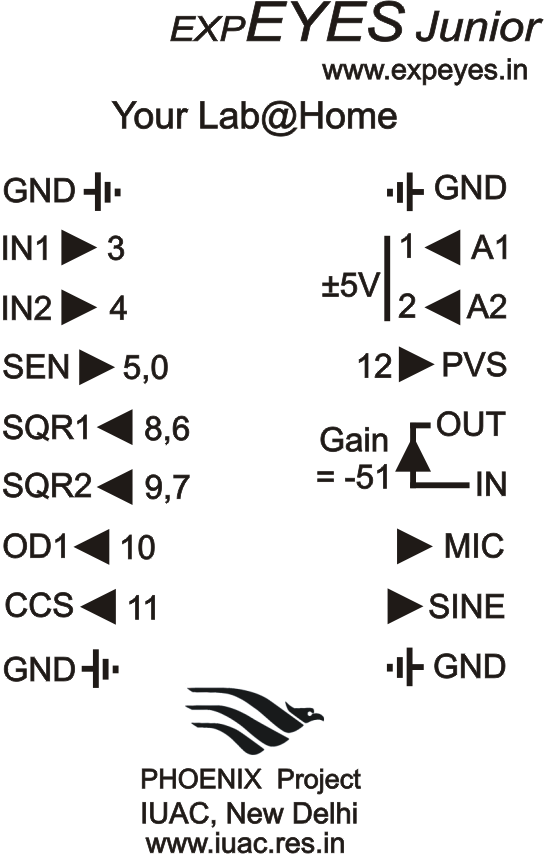
\includegraphics[width=5cm]{pics/top-panel} 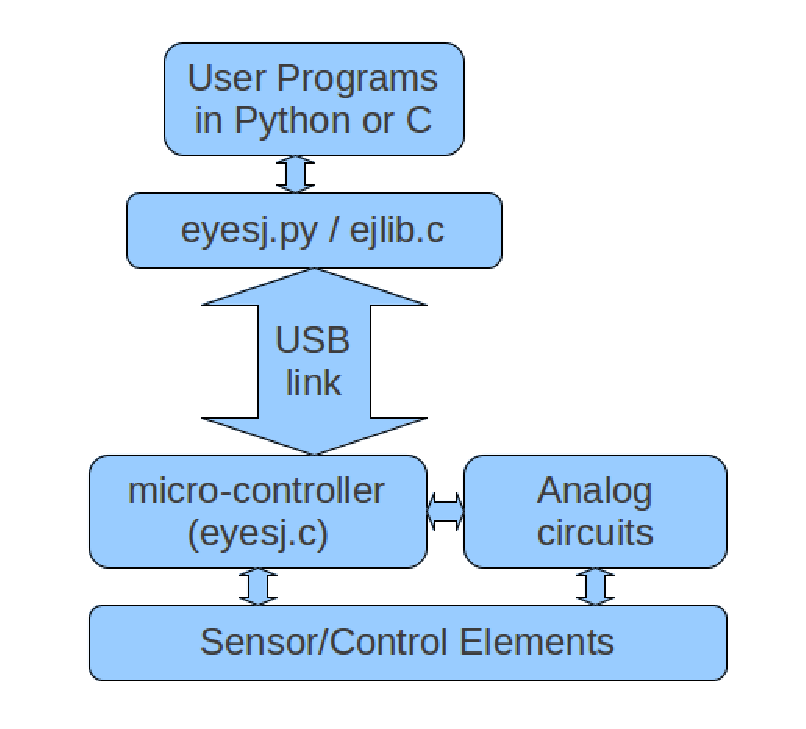
\includegraphics[width=6cm]{pics/eyesjun-block}
\par\end{centering}

\caption{expEYES Junior Top panel and Block diagram\label{fig:expEYES-Junior-Top}}
\end{figure}


\begin{table}
\begin{tabular}{|c|c|c|}
\hline 
Pin \# & Name & Description\tabularnewline
\hline 
\hline 
1 & GND & Ground\tabularnewline
\hline 
2 & IN1 & 0 to 5V range Analog /Digital Input, Current Source\tabularnewline
\hline 
3 & IN2 & 0 to 5V range Analog / Digital Input, Current Source\tabularnewline
\hline 
4 & SEN & 0 to 5V range Analog/Digital Input, with 5K pullup, for resistive
sensors\tabularnewline
\hline 
5 & SQR1 & .7Hz to 200kHz Square Wave Output, $100\Omega$ series resistor\tabularnewline
\hline 
6 & SQR2 & .7Hz to 200kHz Square Wave Output, no series resistor\tabularnewline
\hline 
7 & OD1 & Digital Output, no series resistor\tabularnewline
\hline 
8 & CCS & 1 mA Constant Current Source with ON/OFF Control\tabularnewline
\hline 
9 & GND & Ground\tabularnewline
\hline 
10 & GND & Ground\tabularnewline
\hline 
11 & SINE & Sinewave output, around 150 Hz, 4 volts\tabularnewline
\hline 
12 & MIC & Output of the microphone, amplified 51 times\tabularnewline
\hline 
13 & IN & Inverting Amplifier Input, maximum gain = 51\tabularnewline
\hline 
14 & OUT & Amplifier output, of Pin13\tabularnewline
\hline 
15 & PVS & Programmable Voltage Output, from 0 to 5 volts.\tabularnewline
\hline 
16 & A2 & $\pm5V$ range Analog Input\tabularnewline
\hline 
17 & A1 & $\pm5V$ range Analog Input\tabularnewline
\hline 
18 & GND & Ground\tabularnewline
\hline 
\end{tabular}

\caption{Description of Input/Output Terminals\label{tab:Description-of-Input/Output}}
\end{table}



\section{Software}

There are mainly three modules under the expeyes package:
\begin{itemize}
\item eyesj.py : hardware communication
\item eyeplot.py : Graphics using using Tkinter module
\item eyemath.py : data analysis using modules numpy and scipy
\item ejlib.c \& ejlib.h : C library and the header file
\end{itemize}
They can be installed by using the .tgz files or the .deb packages
provided on http://expeyes.in.


\chapter{Hardware Communication}

The module expeyes.py contains all the functions required for communicating
to the hardware in addition to some utility functions. The functions
are inside a class and the open() function returns an object of this
class if expEYES hardware is detected. After that the function calls
to access expEYES are done using this object, as shown in the example
below.
\begin{lyxcode}
import~expeyes.eyesj~~~~~~\#~import~the~eyes~library

p~=~expeyes.eyesj.open()~~\#~returns~an~object~if~hardware~is~found

print~p.get\_voltage(1)~~~~\#~print~the~voltage~at~input~A1
\end{lyxcode}
A sample program in C language is given below. This should be compiled
and executed.
\begin{lyxcode}
\#include~\textquotedbl{}ejlib.c\textquotedbl{}

int~fd;

int~main()~

~~~\{

~~~byte~ss{[}10{]};~

~~~fd~=~open\_eyesj();~

~~~if(fd~<~0)~

~~~~~\{

~~~~~fprintf(stderr,\textquotedbl{}EYES~Open~Failed\textbackslash{}n\textquotedbl{});

~~~~~exit(0);

~~~~~\}

~~~if(get\_version(ss)~!=~0)~exit(1);

~~~printf(``\%s\textbackslash{}n'',ss);

\}
\end{lyxcode}
On error, the Python functions returns None (-1 in the case of time
interval measurements). On success the data is returned. The C functions
returns zero on success, en errorcode otherwise. The data is always
returned using the addresses passed to the function by the calling
program. In both Python and C, the functions are given the same names.
The main difference is in returning the results. In C, you need to
pass an address for that. The function returns only the status of
the operation. Some of the C functions are mentioned below. It is
easier to have a look at the header file \textit{ejlib.h}.

For every function, the Python and C versions are described, but no
example code given in C. Every function communicates to the program
running on the micro-controller on the expEYES Junior board. The hardware
communication functions can be broadly grouped into analog inputs,
analog outputs, digital inputs, digital outputs, time interval measurements,
waveform generation etc. For plotting data from expEYES, the python-matplotlib
package is used.

The following sections will introduce features of expEYES with examples.
The voltages applied MUST be within the specified limits. \emph{A
channel number is assigned to identify every Analog/Digital signal.
The function calls uses this number for accessing it.}

\begin{table}
\begin{centering}
\begin{tabular}{|c|c|}
\hline 
Channel \# & Name\tabularnewline
\hline 
\hline 
0 & Analog Comparator output\tabularnewline
\hline 
1 & A1\tabularnewline
\hline 
2 & A2\tabularnewline
\hline 
3 & IN1\tabularnewline
\hline 
4 & IN2\tabularnewline
\hline 
5 & SEN\tabularnewline
\hline 
6 & SQR1 readback\tabularnewline
\hline 
7 & SQR2 readback\tabularnewline
\hline 
8 & SQR1 output\tabularnewline
\hline 
9 & SQR1 output\tabularnewline
\hline 
10 & OD1 output\tabularnewline
\hline 
11 & CCS output control\tabularnewline
\hline 
12 & PVS Readback\tabularnewline
\hline 
\end{tabular}
\par\end{centering}

\caption{Signals and Channel Numbers\label{tab:Signals-and-Channel}}
\end{table}



\section{Analog Output}

The Programmable Voltage Sources (PVS) can be set anywhere between
0 and 5 volts. The resolution is 12 bits, means the minimum step is
5000/4095, around 1.25 millivolts.


\subsection{set\_voltage()}

Set the output voltage of the PVS. The value of \textit{V} should
be in 0 to 5 volts range. The function returns the actual value set,
by reading it back using an ADC input (channel number 12). 
\begin{lyxcode}
print~p.set\_voltage(2.5)~~~~~~\#~Sets~2.5~volts~on~PVS
\end{lyxcode}

\paragraph*{C function:}

byte set\_voltage(float v, float{*} vset); // vset returns the readback
of PVS


\section{Digital Inputs (IN1, IN2 and SEN)}

You can connect them externally to GND or 5 volts , to make the voltage
level HIGH or LOW. Any voltage less than 1 volt is taken as a LOW
or 0. Anything greater than 2.5 volts is treated as a HIGH or 1. These
terminals can also be configured as Analog Inputs. 


\subsection{get\_state(channel\#)}

Returns 0 or 1, depending on the voltage level at the input pin
\begin{lyxcode}
print~p.get\_state(3)~~~~\#~prints~logic~level~of~IN1.~~IN2~=~4,~SEN~=~5

print~p.get\_state(0)~~~~\#~Returns~``1''~if~SEN~>~1.25~volts
\end{lyxcode}
Channel 0 represents the analog comparator output. The positive input
of analog comparator should be connected to SEN. Negative input is
internally connected to 1.25 volts.

One of the powerful feature of digital inputs is the ability to measure
the time between level transitions with microsecond resolution. This
will be discussed later.


\paragraph*{C function:}

byte get\_state(byte pin, byte {*}st); // variable st returns 0 or
1.


\section{Digital Output (OD1)}

You can set the voltage level on them to LOW or HIGH volts using software.
If you connect LEDs to them, use a 1K$\Omega$ series resistor for
current limiting.


\subsection{set\_state(channel\#, state)}

This function sets the specified channel to state ``0'' or ``1''.
\begin{lyxcode}
p.set\_state(10,1)~~~~\#~Sets~OD1~HIGH.~Channel~number~of~OD1~is~10
\end{lyxcode}
The outputs SQR1 (8) and SQR2 (9) also can behave as digital outputs,
provided they are not configured to generate Square or PWM outputs.


\paragraph*{C function:}

byte set\_state(byte pin, byte state); // pin is set to 0 or 1, according
to the value of state.


\section{Analog Inputs (A1,A2,IN1,IN2 \& SEN)}

The analog inputs A1 and A2 accept voltages between -5 volts and +5
volts. The Inputs IN1, IN2 and SEN can accept voltages in the 0 to
5 volts range. We can read the voltage level at any of this inputs,
either as single reads or multiple reads in a single function call,
normally to capture a waveform. The time interval between consecutive
reads within a capture can be set with microsecond resolution.


\subsection{get\_voltage(channel\#)}
\begin{lyxcode}
print~p.get\_voltage(1)~~\#~voltage~at~A1

print~p.get\_voltage(2)~~\#~voltage~at~A2

print~p.get\_voltage(3)~~\#~voltage~at~IN1

print~p.get\_voltage(4)~~\#~voltage~at~IN2

print~p.get\_voltage(5)~~\#~voltage~at~SEN

print~p.get\_voltage(6)~~\#~voltage~at~SQR1~output

print~p.get\_voltage(7)~~\#~voltage~at~SQR2~output

print~p.get\_voltage(12)~\#~voltage~at~PVS~output
\end{lyxcode}
Connect PVS to A1 using a piece of wire and run the following program
several times.
\begin{lyxcode}
import~expeyes.eyesj~~~~

p~=~expeyes.eyesj.open()

v~=~input('Enter~V~(0~to~5)')

print~p.set\_voltage(v)~~~\#~prints~the~voltage~set~on~PVS

print~p.get\_voltage(1)~~~\#~voltage~at~A1
\end{lyxcode}
If the voltages are in the 0 to 5 volts range, use IN1 or IN2 for
better results. The $\pm5V$ range inputs A1 \& A2 are converted in
to 0 to 5V range using summing junctions. The amplifiers used for
this will have some gain and offset errors. The resolution also is
halved because of the doubles total range. The input SEN has a 5k
pullup resistor to 5 volts, for connecting photo-transistors and other
resistive sensors . 


\paragraph*{C function:}

byte get\_voltage(byte ch, float{*} v)


\subsection{get\_voltage\_time(channel\#)}

This function returns the time stamp, from the PC clock, and the voltage
in a tuple. This is useful for data logging applications. 


\paragraph*{C function:}

byte get\_voltage(byte ch, int{*} t, float{*} v)


\subsection{get\_voltageNS(channel\#)}

The \emph{get\_voltage()} function mentioned in the previous section
measures the voltage after putting the micro-controller is SLEEP mode,
for better accuracy. This will stop waveforms set on SQR1 \& SQR2.
If that is not accepatble for a particular experiment, one can use
this function.
\begin{lyxcode}
print~p.get\_voltageNS(1)~~\#~voltage~at~A1
\end{lyxcode}

\paragraph*{C function:}

byte get\_voltageNS(byte ch, float{*} v)


\subsection{capture(ch, NP, tg)}

The argument \textit{ch} is the input channel number, \textit{NP}
is the number of measurements and \textit{tg} is the time between
two measurements in microseconds. Two lists containing the time (milliseconds)
and voltage (volts) coordinates are returned by this function. Capture
calls return analog data with 8 bit resolution. Maximum value of NP
is 1800, limited by the micro-controller RAM available. 

The minimum value of 'tg' is 4 microseconds. The value of 'tg' is
decided by the frequency of the signal to be captured. For example,
one cycle of a 1kHz sine wave is 1000 microseconds. A tg of 20 will
give 50 data points per cycle.

Connect SINE to A1 and run the following program.
\begin{lyxcode}
from~pylab~import~{*}

import~expeyes.eyesj

p~=~expeyes.eyesj.open()

t,v~=~p.capture(1,300,100)

plot(t,v)~~~~~\#~from~pylab

show()~~~~~~~~\#~from~pylab



\begin{tabular}{|c|c|c|}
\hline 
Terminal & Channel \# & Range(V)\tabularnewline
\hline 
\hline 
A1 & 1 & -5 to +5\tabularnewline
\hline 
A2 & 2 & -5 to +5\tabularnewline
\hline 
IN1 & 3 & 0 to 5\tabularnewline
\hline 
IN2 & 4 & 0 to 5\tabularnewline
\hline 
SEN & 5 & 0 to 5\tabularnewline
\hline 
SQR1(read) & 6 & 0 to 5\tabularnewline
\hline 
SQR2(read) & 7 & 0 to 5\tabularnewline
\hline 
\end{tabular}
\end{lyxcode}
If the voltage to be measured is in the 0 to 5V range, use IN1 or
IN2, for a better resolution. The SEN input has a 5$k\Omega$ pullup
resistor to 5V supply. We can calculate the value of a resistance
connected from SEN to GND, from the measured voltage, using Ohm's
law.


\paragraph*{C function:}

byte capture(int ch, int ns, int tg, float{*} data); 

The variable data returns an array of 2{*}ns float type elements,
first ns time coordinates and after that ns voltage coordinates. It
is the responsibility of the calling program to pass the address of
an array having sufficient size. capture\_hr() also returns data in
the same format.


\subsection{capture2, capture3 \& capture4}

These functions captures multiple channels together, with timing correlation.
The maximum value of NP for capture4 = 1800/4 = 450. The minimum value
of 'tg' is 4 microseconds per channel, capture4 should have a minimum
tg of 16.
\begin{lyxcode}
t1,v1,t2,v2~=~capture2(ch1,~ch2,~NP,~tg)

t1,v1,t2,v2~=~capture2\_hr(ch1,~ch2,~NP,~tg)

t1,v1,t2,v2,t3,v3~=~capture3(ch1,~ch2,~ch3,~NP,~tg)

t1,v1,t2,v2,t3,v3,t4,v4~=~capture4(ch1,~ch2,~ch3,~ch4,~NP,~tg)
\end{lyxcode}

\paragraph*{C function:}

byte capture2(int ch1, int ch2, int ns, int tg, float{*} data); 

The variable data returns an arrays of 2(2{*}ns) float type elements.
First (2{*}ns) are the time and voltage values for channel 1 and the
next (2{*}ns) for channel 2. Function capture3 and capture4 also returns
data in a similar manner.


\subsection{capture\_hr(ch, NP, tg), capture2\_hr(ch1, ch2, NP, tg)}

These two functions captures data with higher resolution (12 bits).
In this case each value takes 2 bytes and the maximum value of NP
is 900 for capture\_hr, and 450 for capture2\_hr. High resolution
version is NOT available for capture3 and capture4.
\begin{lyxcode}
t1,v1~=~capture\_hr(ch1,~900,~10)

t1,v1,t2,v2~=~capture2\_hr(ch1,~ch2,~450,~20)

plot(t1,v1,~t2,v2)

show()
\end{lyxcode}
We can find out the amplitude and frequency of the input waveform
by mathematically fitting the captured data to the equation of a sine
wave$V=V_{0}\sin\left(2\pi ft+\theta\right)+C$ . By capturing 4 to
5 cycles, the frequency can be obtained within 0.1\% error.


\section{Capture modifiers}

When a periodic wave form is captured, the starting point could be
at any voltage, within the minimum and maximum voltage. To implement
an oscilloscope, we need to make sure that the starting point is always
same, else the trace will be jumping around. This is a simple example
of a capture modifier. expEYES implements several other types of capture
modifiers to enhance the functionality of the capture functions. The
basic idea is to perform some action just before starting the waveform
capture. The important types of modifiers (or actions) are
\begin{itemize}
\item Analog Trigger on any input channel, trigger level can be set by the
user.
\item Wait for HIGH, LOW, Falling Edge or Rising Edge on Inputs IN1, IN2,
SEN, SQR1 or SQR2
\item Set, Clear or send Pulse one of the Digital Outputs, mainly OD1. SQR1
\& SQR2 also will act as digital outputs if frequency is set to zero.
\end{itemize}
\begin{table}
\begin{centering}
\begin{tabular}{|c|c|c|}
\hline 
Action & Code & Description\tabularnewline
\hline 
\hline 
AANATRIG & 0 & Trigger on analog input level\tabularnewline
\hline 
ASET & 1 & Makes the specified Output HIGH\tabularnewline
\hline 
ACLR & 2 & Makes the specified Output LOW\tabularnewline
\hline 
APULSEHT & 3 & Send High True Pulse on Output \tabularnewline
\hline 
APULSELT & 4 & Send Low True Pulse on Output\tabularnewline
\hline 
AWAITHI & 5 & Wait for HIGH level on specified Input\tabularnewline
\hline 
\multicolumn{1}{|c|}{AWAITLO} & 6 & Wait for LOW level on specified Input\tabularnewline
\hline 
AWAITRISE & 7 & Wait for Rising Edge on specified Input\tabularnewline
\hline 
AWAITFALL & 8 & Wait for Falling Edge on specified Input\tabularnewline
\hline 
\end{tabular}
\par\end{centering}

\caption{Capture Modifiers\label{tab:Capture-Modifiers}}
\end{table}


enable\_action(action, Selected I/O) is the function call for registering
actions. They will be valid on subsequent capture calls. Calling disable\_actions()
removes all registered actions and capture goes back to its default
state of analog triggering on the captured channel. For convenience,
we have defined more functions that internally call the function enable\_action()


\subsection{set\_trigger(trigval)}

Sets the analog voltage trigger level, for the capture function. If
the specified voltage value is not found at the input, within the
timeout period, the capture is done ignoring the trigger condition.
\begin{lyxcode}
p.set\_trigger(2048)~~~\#~0~to~4095~is~the~analog~range
\end{lyxcode}

\subsection{set\_trigsource(channel\#)}

The Input source to be used for analog level triggering. It need not
be the one that is captured. The example code below demonstrates the
effect of this function. Connect SINE to A1 before running.
\begin{lyxcode}
from~pylab~import~{*}

import~expeyes.eyesj

p~=~expeyes.eyesj.open()

ts~=~1~~~~~~\#~run~the~program~by~changing~this~to~2

p.set\_trig\_source(ts)

t,v~=~p.capture(1,300,50)

plot(t,v)

t,v~=~p.capture(1,300,50)

plot(t,v)

show()
\end{lyxcode}
The traces will not overlap if the trigger source is set to some other
channel, provided there is no time correlation between the two inputs.


\paragraph*{C function:}

byte set\_trig\_source(byte ch);


\subsection{enable\_wait\_high(channel\#), ...\_low(...), ...\_falling(...),
...\_rising(...)}

Calling this function makes all the subsequent \textbf{capture} calls
to wait for a HIGH / LOW / rising edge/ falling edge, on the specified
input before starting the digitization.
\begin{lyxcode}
p.enable\_action(1,~11)~~~~\#~Start~CCS~before~capturing

p.enable\_wait\_rising(3)~~~\#~wait~for~a~rising~edge~on~IN1

p.disable\_actions()~~~~~~~\#~removes~all~modifiers
\end{lyxcode}

\paragraph*{C function:}

byte enable\_wait\_high(byte ch);


\subsection{enable\_set\_high(channel\#), ...\_low(...), ...\_pulse\_high(...),
...\_low(...)}

In some applications, it would be necessary to make a digital output
high/low or send a pulse, width set by another function, with before
digitization starts. Capturing the voltage across a capacitor while
charging / discharging is a typical application of this feature. Connect
a 1uF capacitor between A1 and GND. Connect a 1K$\Omega$ resistor
from OD1 to A1 and run the following code.
\begin{lyxcode}
from~pylab~import~{*}

import~expeyes.eyesj

p~=~expeyes.eyesj.open()

p.set\_state(10,1)~~~~~~~~\#~Take~OD1~HIGH

p.enable\_set\_low(10)~~~~~\#~OD1~go~LOW~before~capture

t,v~=~p.capture(1,200,20)

plot(t,v)

show()
\end{lyxcode}

\paragraph*{C function:}

byte enable\_set\_high(byte ch);


\subsection{set\_pulsewidth(width)}

Sets the width of the pulse that is send on the digital outputs before
capturing, in microseconds, up to 250.
\begin{lyxcode}
p.set\_pulsewidth(100)~~\#~sets~the~pulsewidth
\end{lyxcode}

\paragraph*{C function:}

byte set\_pulsewidth(u16 width);


\section{Waveform Generation}

ExpEYES can generate square waves on SQR1 and SQR2. The frequency
can vary from 0.7 Hz to 100 kHz. All intermediate values are NOT possible
since the output is generated by timers and comparators. The function
returns the actual values set, closest possible to the requested.
Output SQR1 has a $100\Omega$ series resistor for current limiting,
but SQR2 is directly connected.


\subsection{set\_sqr1(freq), set\_sqr2(freq)}

Generates a square waveform, having 50\% duty cycle, on SQR1/SQR2.
SQR1 has a 100$\Omega$ series resistor on it. Setting freq = 0 will
make the output HIGH and setting freq = -1 will make it LOW. Both
these cases disables the Timer/Counter and configures it as a normal
digital output.
\begin{lyxcode}
import~expeyes.eyesj~~~~

p~=~expeyes.eyesj.open()

print~p.set\_sqr1(1000)~
\end{lyxcode}

\paragraph*{C function:}

byte set\_sqr1(float freq, float {*}fset);

The desired value is specified in 'freq', after the call 'fset' will
contain the actual frequency set.


\subsection{set\_sqrs(freq, phase shift in percent)}

Generates a square waveform of same frequency on both SQR1 and SQR2.
The phase shift between the two can be set in percentage of the Time
Period.
\begin{lyxcode}
p.set\_sqrs(1000,50)~~~~\#~Two~out~of~phase~waveforms~
\end{lyxcode}

\paragraph*{C function:}

byte set\_sqrs(float freq, float diff, float {*}fset);


\subsection{set\_sqr1\_pwm(dutycycle), set\_sqr2\_pwm(dutycycle)}

SQR1 and SQR2 can be configured for making Pulse Width Modulated waveform.
The duty cycle is specified in percentage. The frequency is 488Hz
by default, because the second argument is set to 14 by default. This
is the index of counter's bit which triggers the PWM. Specifying the
second argument can be used for changing the frequency. Reducing it
by 1 will double the frequency and increasing by 1 will halve it.
\begin{lyxcode}
print~p.set\_sqr1\_pwm(20)~~~~~~\#~488Hz,~20\%~duty~cycle~

print~p.set\_sqr1\_pwm(50,~15)~~\#~244Hz,~50\%~duty~cycle

print~p.set\_sqr1\_pwm(50,~13)~~\#~976Hz,~50\%~duty~cycle~
\end{lyxcode}

\paragraph*{C function:}

byte set\_sqr1\_pwm(byte dc);


\subsection{set\_sqr1\_dc(voltage), set\_sqr2\_dc(voltage)}

SQR1 and SQR2 can be configured to generate a DC voltage, by external
filtering, from a PWM waveform. The voltage, 0 to 5V range, is specified
as the argument.
\begin{lyxcode}
print~p.set\_sqr1\_dc(2)~~~\#~7.8~kHz,~40\%~duty~cycle~
\end{lyxcode}
Filtering the waveform generates a DC voltage. Connect 10k from SQR1
to IN1 and 100uF from IN1 to GND.
\begin{lyxcode}
print~p.get\_voltage(3)~~~\#~voltage~at~IN1
\end{lyxcode}
The output voltage depends on the supply voltage provided by USB.
Setting 3 volts means only setting 60\% of the supply voltage. The
readout from IN1 will give the correct value.


\paragraph*{C function:}

byte set\_sqr1\_dc(float volt)


\subsection{get\_frequency(pin)}

Measure the frequency of a 0 to 5V square wave connected to IN1, IN2
or SEN. You can also measure the frequency of SQR1 \& SQR2 outputs
from channels 6 and 7 respectively. Connect SQR1 to IN1 and run the
following code
\begin{lyxcode}
import~expeyes.eyesj~~~~

p~=~expeyes.eyesj.open()

p.set\_sqr1(1000)

print~p.get\_frequency(3)~~~~~~\#~frequency~of~squarewave~at~IN1

print~p.get\_frequency(6)~~~~~~\#~frequency~of~SQR1,~same~as~above
\end{lyxcode}

\paragraph*{C function:}

byte get\_frequency(byte pin, float {*}fr)


\section{Infrared Transmission}

The SQR1 output supports two types of 38kHz infrared transmission
protocol. One is a non-standard 1 byte transmission, that can be received
by another program running on an ATmega32 micro-controller. This can
be used for controlling some device from expEYES junior.


\subsection{irsend1(byte)}

Sends the byte over SQR1. Just connect an IR LED from SQR1 to GND
and issue the command.

To signify a start 38kHz is kept on for 9000 microseconds followed
by a silence of 4400 microseconds. After that 38kHz is kept ON for
680 usec followed by (a) silence of 1560 usecs to transmit a 1 and
440 usecs to transmit a 0. This process is repeated 8 times, starting
with the MSB of the byte to be transmitted. The sequence ends by transmitting
a 340 usecs long burst again. This is received by a program%
\footnote{http://expeyes.in/sites/default/files/debs/recv.c%
} given on the website.

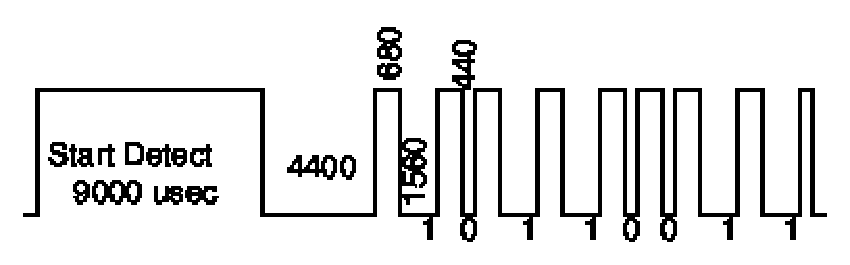
\includegraphics[height=1.5cm]{schematics/ir-code}


\subsection{irsend4(byte, byte, byte, byte)}

The Start and End are identical to irsend1() but instead of 1 byte,
4 bytes are sent in a single transmission. If the numbers are chosen
properly, you can control TVs or other instruments using this.


\section{Passive Time Interval Measurements}

Digital Inputs can be used for measuring time intervals between level
transitions on the digital inputs with microsecond resolution. The
transitions defining the start and finish could be on the same terminal
or on different ones.


\subsection{r2ftime(pin1, pin2) , f2rtime(pin1, pin2)}

r2ftime returns delay in microseconds from a rising edge on pin1 to
a falling edge on pin2, the channel numbers corresponding to the inputs
should be given as the arguments. The pins could be same or distinct.
Similarly f2rtime() measures time from a falling edge to a rising
edge.

Connect SQR1 to IN1 and run the following code, should print around
500 usecs.
\begin{lyxcode}
import~expeyes.eyesj~~~~

p~=~expeyes.eyesj.open()

p.set\_sqr1(1000)~~~~~~~~\#~1kHz,~T=1msec.~half~period~=~500~usecs

print~p.r2ftime(3,3)
\end{lyxcode}

\paragraph*{C function:}

byte r2ftime(byte pin1, byte pin2, float {*}ti)


\subsection{r2rtime(pin1, pin2), f2ftime(pin1, pin2)}

r2rtime returns delay in microseconds from a rising edge to rising
edge. The pins should NOT be the same. The following code shows how
to use this for measuring delay between two transitions.
\begin{lyxcode}
import~expeyes.eyesj~~~~

p~=~expeyes.eyesj.open()

p.set\_sqrs(1000,~25)~~~~~~\#~1000Hz~on~both~SQR1~\&~2.~Delay~by~25\%,~250us

print~p.r2rtime(6,7)~~~~~~\#~Channels~6~\&~7~are~readback~of~SQR1~and~SQR2
\end{lyxcode}

\subsection{multi\_r2rtime(channel\#,skip\_edges)}

Measures time interval between two rising edges of a waveform applied
to a digital input. The second argument is the number of rising edges
to be skipped between the two measured rising edges. This way we can
decide the number of cycles to be measured.

Connect SQ1to IN1 and run the following code.
\begin{lyxcode}
import~expeyes.eyesj~~~~

p~=~expeyes.eyesj.open()

p.set\_sqr1(1000)

a~=~p.multi\_r2rtime(3)~~~~~~\#~time~for~1~cycle~in~usecs

b~=~p.multi\_r2rtime(3,9)~\#~time~for~10~cycles~in~usecs

print~10.0e6/a~~\#~frequency~in~Hz


\end{lyxcode}
For a periodic waveform input, the fourth line of the program returns
the time for one cycle and the fifth one returns the time for 10 cycles
( 9 rising edges in between skipped). This call can be used for frequency
measurement. The accuracy can be improved by measuring larges number
of cycles.


\paragraph*{C function:}

byte multi\_r2rtime(byte pin, byte skip, float {*}ti)


\section{Active Time Interval Measurements}

During some experiments, we need to initiate some action and measure
the time interval to the result of of that action. These functions
are used in experiments like gravity by time of flight and velocity
of sound using ultrasound piezo discs.


\subsubsection{set2rtime (Digital Output, Digital Input)}

This makes the specified Digital Output HIGH and waits for a HIGH
on the Digital Input. Connect a 1k resistor from OD1 to IN1 and a
1uF capacitor from IN1 to GND. 
\begin{quotation}
\begin{flushleft}
p.set2rtime(10, 3)
\par\end{flushleft}
\end{quotation}

\subsubsection{htpulse2rtime(Digital output, Digital Input)}
\begin{lyxcode}
int~htpulse2rtime(out,~in)
\end{lyxcode}
Sends out a single High True pulse on \textbf{out} (SQR1, SQR2 or
OD1) and waits for a rising/falling edge on \textbf{in} (IN1, IN2
or SEN). The duration of the pulse is set by set\_pulsewidth(). On
powerup the width is 13 microseconds. The initial level of \textbf{out}
should be set according to the kind of pulse.

Similarly we have htpulse2ftime(), ltpulse2rtime() and ltpulse2ftime().
\begin{lyxcode}
p.set\_pulse\_width(1)

print~p.htpulse2rtime(10,~3)~
\end{lyxcode}
measures the time from a 1usec wide High True pulse on OD1 to a rising
edge on IN1.


\subsubsection{set\_pulse\_width(width)}

Sets the pulse width, in microseconds, to be used by the htpulse2rtime(),
htpulse2ftime(), ltpulse2rtime(), ltpulse2ftime() functions.
\begin{lyxcode}
p.set\_pulse\_width(10)
\end{lyxcode}

\section{1mA Current Source}

The 1mA constant current can be switched ON or OFF by channel number
11, as shown below
\begin{lyxcode}
p.set\_state(11,~1)~~~~\#~switch~on~CCS~
\end{lyxcode}
We can plot the linear charging of a 1uF capacitor by conecting it
between CCS and GND, and running the following code. Connect CCS to
IN1 for voltage measurement.
\begin{lyxcode}
from~pylab~import~{*}~

import~expeyes.eyesj,~time~

p~=~expeyes.eyesj.open()

p.set\_state(11,0)~~~~~~\#~switch~of~CCS

time.sleep(1)~~~~~~~~~~\#~wait~for~discharge

p.enable\_set\_high(11)~~\#~enable~CCS~just~before~capture~~~

t1,v1=~p.capture\_hr(3,500,10)~

plot(t1,v1)~

show()
\end{lyxcode}

\section{Capacitance measurements}

The IN1 pin can be used for measuring capacitance, ranging from hundred
to several thousand pico Farads. This is done using an internal programmable
constant current source. 


\subsection{measure\_cap()}

Connect the capacitor between IN1 and ground and run the function
measure\_cap().
\begin{lyxcode}
import~expeyes.eyesj

p~=~expeyes.eyesj.open()

print~p.measure\_cap()
\end{lyxcode}
The capacitance is measured by charging the capacitor with a 5.5 uA
constant current source for a fixed duration. The total charge is
given by Q = It = CV. If V,I and t are known, C can be calculated.
The value of the current source may vary from 5.5 uA and the empty
socket, along with tracks, also has some capacitance. These error
are taken can by calibrating it using a known capacitor. The error
factors are stored in EEPROM of the micro-controller.


\subsection{measure\_cv(channel, duration, current)}

This is a more flexible version of measure\_cap, allowing to set the
current source on IN1 or IN2. The current source is activated for
'duration' microseconds. The last argument could be .55, 5.5, 55 or
550 microamps. The function returns the voltage at the selected input
after applying the current for the specified duration.

Depending on the value of the capacitor connected, we need to select
duration and current such that the voltage developed is between 2
to 4 volts for good results. Connect a 330 pF capacitor from IN1 to
GND and run the following code.
\begin{lyxcode}
import~expeyes.eyesj

p~=~expeyes.eyesj.open()

print~p.measure\_cv(3,~200,~5.5)~~\#~result~was~3.017~volts
\end{lyxcode}
The capacitance can be calculated using the expressions Q =CV and
Q = I{*}t. C =I{*}t/v = 5.5{*}200/3.017 = 364 pF. Subtracting the
Stray capacitance 32pF gives a result of 332pF.


\subsection{set\_current(channel, current)}

This function enables the internal current source on IN1 or IN2. This
Constant Current Source may be used for measuring the current with
some other device. The voltage readback is not working as expected.
Using an ammeter connected from IN1 to ground, it is found that the
current is 5.5 uA , 47 uA and 450 uA, somewhat less than the specification,
in higher ranges.


\section{Resistance Measurements}

The SEN input is internally connected to 5 volts through a 5100$\Omega$
resistor. It is possible to calculate the value of a resistor connected
from SEN to GND using Ohm's law. However, the internal resistor may
not be exactly 5100 due to component tolerance.


\subsection{measure\_res()}

The input SEN is connected to 5 volts internally through a 5100 Ohm
resistor. Connecting an external resistor from SEN to GND makes a
potential divider. It is possible to calculate the value of the resistor
connected using Ohm's law.

This function returns the value of a resistance connected from SEN
to GND, calculated using the equation

$R_{ext}=R_{int}*V{}_{SEN}/(5.0-V_{SEN})$


\section{Disk Writing}


\subsection{save\_data}

Input data is of the form, {[} {[}x1,y1{]}, {[}x2,y2{]},....{]} where
x and y are vectors, are save to a text file.

Save the data returned by the capture functions into a text file.
Default filename is `plot.dat', that can be overriden by the second
argument. Connect SINE to A1 and run the following code.
\begin{lyxcode}
import~expeyes.eyesj~~~~

p~=~expeyes.eyesj.open()

t,v~=~p.capture(1,~200,~100)

p.save({[}{[}t,v{]}{]},~'sine.dat')
\end{lyxcode}
open the file using the command 

\$xmgrace sine.dat


\chapter{Data processing}

The data acquired from expEYES hardware is analyzed using various
mathematical techniques like least-square fitting, Fourier transform
etc. The module named eyemath.py does this with the help of functions
from the 'scipy' package. Most of the functions accepts the data format
returned by capture functions. 


\subsection{fit\_sine}

Accepts two vectors {[}x{]} and {[}y{]} and tries to do a least-square
fitting of the data with the equation $A\sin\left(2\pi ft+\theta\right)+C$.
Returns the fitted data and the parameter list$[A,f,\theta,C]$. Connect
SINE to A1 and run the following code.
\begin{lyxcode}
from~pylab~import~{*}

import~expeyes.eyesj,~expeyes.eyemath~as~em

p~=~expeyes.eyesj.open()

t,v=~p.capture(1,400,100)

vfit,~par~=~em.fit\_sine(t,v)

print~par~~~~~~~~\#~$A,f,\theta,C$

plot(t,v)~~~~~~~~\#~The~raw~data

plot(t,vfit)~~~~~\#~data~calculated~from~par

show()
\end{lyxcode}
par{[}1{]} is frequency in kHz, since the time is given in milliseconds.


\subsection{fit\_dsine}

Accepts two vectors {[}x{]} and {[}y{]} and tries to do a least-square
fitting of the data with the equation $A=A_{0}\sin\left(2\pi ft+\theta\right)\times exp(-dt)+C$.
Returns the fitted data and the parameter list$[A,f,\theta,C,d]$.
par{[}1{]} is frequency in kHz, since the time is given in milliseconds
and 'd' is the damping factor.


\subsection{fit\_exp}

Accepts two vectors {[}x{]} and {[}y{]} and tries to do a least-square
fitting of the data with the equation $A=A_{0}\exp\left(kt\right)+C$.
Returns the fitted data and the parameter list$[A,k,C]$. Connect
a 1uF capacitor from A1 to GND, 1k$\Omega$ resistor from OD1 to A1
and run the following code.
\begin{lyxcode}
from~pylab~import~{*}

import~expeyes.eyesj,~expeyes.eyemath~as~em

p~=~expeyes.eyesj.open()

p.set\_state(10,1)~~~~~\#~Take~OD1~HIGH

p.enable\_set\_low(10)~~~~\#~OD1~go~LOW~before~capture

t,v~=~p.capture(1,200,20)

plot(t,v)

vfit,~par~=~em.fit\_exp(t,v)

print~par

plot(t,v)~~~~~~~~\#~The~raw~data

plot(t,vfit)~~~~~\#~data~calculated~from~par

show()
\end{lyxcode}
-(1/par{[}1{]}) is the time constant RC in seconds.


\subsubsection{fft}

Does a Fourier transform of a given data set. The sampling interval
in milliseconds is the second argument. Returns the frequency spectrum,
ie. the relative strength of each frequency component. Connect SINE
to A1 and run the following code.
\begin{lyxcode}
from~pylab~import~{*}

import~expeyes.eyesj,~expeyes.eyemath~as~em

ns~=~1000~~~\#~number~of~points~to~be~captured

tg~=~100~~~~\#~time~between~reads~in~usecs

p~=~expeyes.eyesj.open()

t,v=~p.capture(1,~ns,~tg)

x,y~=~em.fft(v,~tg~{*}~0.001)~~\#~tg~in~millisecs

plot(t,v)~~~~~\#~The~raw~data

plot(x,y)~~~~~\#~data~calculated~from~par

show()
\end{lyxcode}
The frequency spectrum should feature a peak at frequency f=150Hz.
A small peak at frequency 2f may be visible.

Modify this program to show the frequency spectrum of a square wave.


\chapter{Experiments }

Most of the experiments described in the user manual can be done by
writing few lines of Python code.


\section{Transient response of LC circuit}

Connect inductor from OD1 to A1, capacitor from A1 to GND. 
\begin{lyxcode}
NP~=~200~~~\#~number~of~readings

tg~=~10~~~~\#~time~gap~between~them,~keep~NP{*}tg~around~3{*}RC

from~pylab~import~{*}

import~expeyes.eyesj,~expeyes.eyemath~as~em

p~=~expeyes.eyesj.open()

p.set\_state(10,1)

p.enable\_set\_low(10)~~~~~~~~~~~\#~OD1~go~LOW~before~capture

t,v~=~p.capture\_hr(1,NP,tg)~~~~\#~choose~NP{*}tg~according~to~time~constant

plot(t,v)

vf,~par~=~em.fit\_exp(t,v)~~~~~~\#~exponential~fit

plot(t,~vf,'r')

print~abs(1./par{[}1{]})~~~~~~~~~~~\#~print~RC~value

show()

\end{lyxcode}

\end{document}
